% Options for packages loaded elsewhere
\PassOptionsToPackage{unicode}{hyperref}
\PassOptionsToPackage{hyphens}{url}
\PassOptionsToPackage{dvipsnames,svgnames,x11names}{xcolor}
%
\documentclass[
  letterpaper,
  DIV=11,
  numbers=noendperiod]{scrartcl}

\usepackage{amsmath,amssymb}
\usepackage{iftex}
\ifPDFTeX
  \usepackage[T1]{fontenc}
  \usepackage[utf8]{inputenc}
  \usepackage{textcomp} % provide euro and other symbols
\else % if luatex or xetex
  \usepackage{unicode-math}
  \defaultfontfeatures{Scale=MatchLowercase}
  \defaultfontfeatures[\rmfamily]{Ligatures=TeX,Scale=1}
\fi
\usepackage{lmodern}
\ifPDFTeX\else  
    % xetex/luatex font selection
\fi
% Use upquote if available, for straight quotes in verbatim environments
\IfFileExists{upquote.sty}{\usepackage{upquote}}{}
\IfFileExists{microtype.sty}{% use microtype if available
  \usepackage[]{microtype}
  \UseMicrotypeSet[protrusion]{basicmath} % disable protrusion for tt fonts
}{}
\makeatletter
\@ifundefined{KOMAClassName}{% if non-KOMA class
  \IfFileExists{parskip.sty}{%
    \usepackage{parskip}
  }{% else
    \setlength{\parindent}{0pt}
    \setlength{\parskip}{6pt plus 2pt minus 1pt}}
}{% if KOMA class
  \KOMAoptions{parskip=half}}
\makeatother
\usepackage{xcolor}
\setlength{\emergencystretch}{3em} % prevent overfull lines
\setcounter{secnumdepth}{-\maxdimen} % remove section numbering
% Make \paragraph and \subparagraph free-standing
\makeatletter
\ifx\paragraph\undefined\else
  \let\oldparagraph\paragraph
  \renewcommand{\paragraph}{
    \@ifstar
      \xxxParagraphStar
      \xxxParagraphNoStar
  }
  \newcommand{\xxxParagraphStar}[1]{\oldparagraph*{#1}\mbox{}}
  \newcommand{\xxxParagraphNoStar}[1]{\oldparagraph{#1}\mbox{}}
\fi
\ifx\subparagraph\undefined\else
  \let\oldsubparagraph\subparagraph
  \renewcommand{\subparagraph}{
    \@ifstar
      \xxxSubParagraphStar
      \xxxSubParagraphNoStar
  }
  \newcommand{\xxxSubParagraphStar}[1]{\oldsubparagraph*{#1}\mbox{}}
  \newcommand{\xxxSubParagraphNoStar}[1]{\oldsubparagraph{#1}\mbox{}}
\fi
\makeatother


\providecommand{\tightlist}{%
  \setlength{\itemsep}{0pt}\setlength{\parskip}{0pt}}\usepackage{longtable,booktabs,array}
\usepackage{calc} % for calculating minipage widths
% Correct order of tables after \paragraph or \subparagraph
\usepackage{etoolbox}
\makeatletter
\patchcmd\longtable{\par}{\if@noskipsec\mbox{}\fi\par}{}{}
\makeatother
% Allow footnotes in longtable head/foot
\IfFileExists{footnotehyper.sty}{\usepackage{footnotehyper}}{\usepackage{footnote}}
\makesavenoteenv{longtable}
\usepackage{graphicx}
\makeatletter
\def\maxwidth{\ifdim\Gin@nat@width>\linewidth\linewidth\else\Gin@nat@width\fi}
\def\maxheight{\ifdim\Gin@nat@height>\textheight\textheight\else\Gin@nat@height\fi}
\makeatother
% Scale images if necessary, so that they will not overflow the page
% margins by default, and it is still possible to overwrite the defaults
% using explicit options in \includegraphics[width, height, ...]{}
\setkeys{Gin}{width=\maxwidth,height=\maxheight,keepaspectratio}
% Set default figure placement to htbp
\makeatletter
\def\fps@figure{htbp}
\makeatother

\KOMAoption{captions}{tableheading}
\makeatletter
\@ifpackageloaded{caption}{}{\usepackage{caption}}
\AtBeginDocument{%
\ifdefined\contentsname
  \renewcommand*\contentsname{Table of contents}
\else
  \newcommand\contentsname{Table of contents}
\fi
\ifdefined\listfigurename
  \renewcommand*\listfigurename{List of Figures}
\else
  \newcommand\listfigurename{List of Figures}
\fi
\ifdefined\listtablename
  \renewcommand*\listtablename{List of Tables}
\else
  \newcommand\listtablename{List of Tables}
\fi
\ifdefined\figurename
  \renewcommand*\figurename{Figure}
\else
  \newcommand\figurename{Figure}
\fi
\ifdefined\tablename
  \renewcommand*\tablename{Table}
\else
  \newcommand\tablename{Table}
\fi
}
\@ifpackageloaded{float}{}{\usepackage{float}}
\floatstyle{ruled}
\@ifundefined{c@chapter}{\newfloat{codelisting}{h}{lop}}{\newfloat{codelisting}{h}{lop}[chapter]}
\floatname{codelisting}{Listing}
\newcommand*\listoflistings{\listof{codelisting}{List of Listings}}
\makeatother
\makeatletter
\makeatother
\makeatletter
\@ifpackageloaded{caption}{}{\usepackage{caption}}
\@ifpackageloaded{subcaption}{}{\usepackage{subcaption}}
\makeatother

\ifLuaTeX
  \usepackage{selnolig}  % disable illegal ligatures
\fi
\usepackage{bookmark}

\IfFileExists{xurl.sty}{\usepackage{xurl}}{} % add URL line breaks if available
\urlstyle{same} % disable monospaced font for URLs
\hypersetup{
  pdftitle={Exercise},
  pdfauthor={Wojciech Hardy},
  colorlinks=true,
  linkcolor={blue},
  filecolor={Maroon},
  citecolor={Blue},
  urlcolor={Blue},
  pdfcreator={LaTeX via pandoc}}


\title{Exercise}
\author{Wojciech Hardy}
\date{2022-03-29}

\begin{document}
\maketitle


\section{Game of Thrones - Season 1 summary in
numbers}\label{game-of-thrones---season-1-summary-in-numbers}

\subsubsection{\texorpdfstring{\textbf{(\emph{Warning:} spoilers
ahead)}}{(Warning: spoilers ahead)}}\label{warning-spoilers-ahead}

\begin{center}\rule{0.5\linewidth}{0.5pt}\end{center}

\subsubsection{Overview}\label{overview}

(From the
\href{https://en.wikipedia.org/wiki/Game_of_Thrones\#Premise}{Wikipedia})
Game of Thrones is an American fantasy drama television series created
by David Benioff and D. B. Weiss for HBO. It is an adaptation of A Song
of Ice and Fire, a series of fantasy novels by George R. R. Martin, the
first of which is A Game of Thrones.

Set on the fictional continents of Westeros and Essos, Game of Thrones
has a large ensemble cast and follows several story arcs throughout the
course of the show. A major arc concerns the Iron Throne of the Seven
Kingdoms of Westeros through a web of political conflicts among the
noble families either vying to claim the throne or fighting for
independence from it. Another focuses on the last descendant of the
realm's deposed ruling dynasty, who has been exiled to Essos and is
plotting a return to the throne. A third story arc follows the Night's
Watch, a military order defending the realm against threats from the
North.

\begin{center}\rule{0.5\linewidth}{0.5pt}\end{center}

\subsubsection{Season 1 summary}\label{season-1-summary}

Season 1 of Game of Thrones consisted of 10 episodes that aired between
April 17 and June 19, 2011 on HBO. The show gathered an average of 2.515
first-day TV viewers in the US, with the number growing from 2.22 to
3.04 million by the end of the season.

The most popular episode of the season was ``Fire and Blood'', in which:

\begin{quote}
``The North secedes from the Seven Kingdoms and proclaims Robb as king.
With Jaime as the Starks' prisoner and Robert's two brothers, Stannis
and Renly, each challenging Joffrey's claim to the throne, Tywin
appoints Tyrion as acting King's Hand, while Tywin fights to defend
Joffrey's reign. Jon attempts to desert the Night's Watch to avenge Ned
and join Robb, but his Night's Watch brothers convince him to honor his
oath. Jon joins an expedition to search for Benjen Stark beyond the
Wall. Yoren, a Night's Watch recruiter, smuggles Arya out of King's
Landing disguised as a boy, while Joffrey intends to crown Sansa his
queen, despite executing her father. Daenerys's baby is born deformed
and dead, and Drogo is left in a vegetative state by the witch's
treacherous magic. Daenerys compassionately ends Drogo's life. She
places the three dragon eggs on Drogo's funeral pyre and sets it afire,
also burning the witch alive. Ignoring Jorah's pleas, she walks into the
flames. When the embers die the following morning, Daenerys is found in
the ashes, unharmed, flanked by three newly-hatched baby dragons. Jorah
and other witnesses kneel before her.''
\end{quote}

\begin{center}\rule{0.5\linewidth}{0.5pt}\end{center}

You can see how the viewership of the episodes changed in Figure 1.

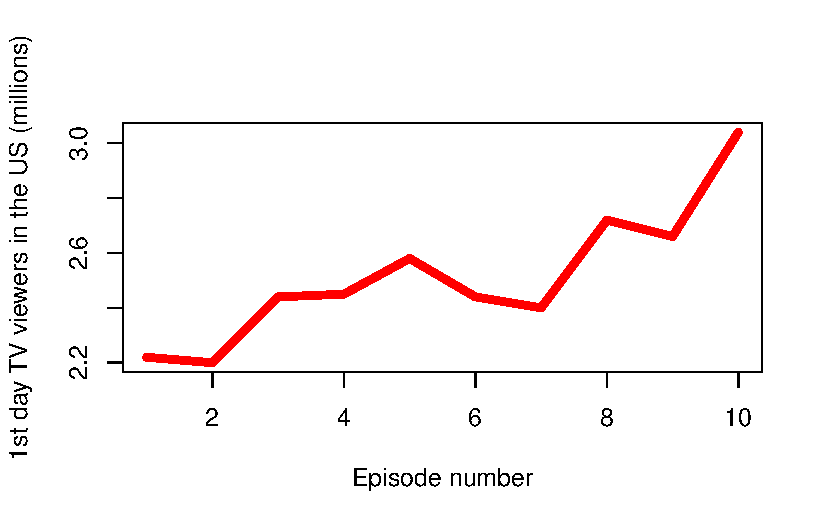
\includegraphics{QMD_Assignment_QM2_files/figure-pdf/viewers_plot-1.pdf}

\begin{center}\rule{0.5\linewidth}{0.5pt}\end{center}

Finally, the episodes with the above-average viewership were:

\begin{longtable}[]{@{}lcc@{}}
\toprule\noalign{}
No.~in season & Title & Directed by \\
\midrule\noalign{}
\endhead
\bottomrule\noalign{}
\endlastfoot
5 & ``The Wolf and the Lion'' & Brian Kirk \\
8 & ``The Pointy End'' & Daniel Minahan \\
9 & ``Baelor'' & Alan Taylor \\
10 & ``Fire and Blood'' & Alan Taylor \\
\end{longtable}




\end{document}
